\chapter{علم الفيروسات}\label{ch:b3:virology}

على الأرض نحو $10^{31}$ جسيم فيروسي، أي عشرة لكل خلية،
وهي تقتل في البحر خُمس البكتيريا كلها كل يوم. \omterm{def:b3:virology:virus}{والفيروس}
ليس خلية: فلا استقلاب له، ولا ريبوزومات، ولا سبيل إلى صنع شيء
بنفسه. وإنما هو جينوم --- قصير كمورّثتين، طويل كألفي
مورّثة --- ملفوف في \omterm{def:b3:virology:virus}{غلاف} بروتيني، يدخل خلية ويحوّل
آلة الخلية إلى صنع نسخ منه. وقد قتلت إنفلونزا عام 1918
خمسين مليون إنسان؛ وأما الجدري، الذي قتل ثلاثمئة
مليون في القرن العشرين وحده، فاستُؤصل عام 1980 بفضل
\omterm{def:b3:virology:drugs}{لقاح} جُرّب أول مرة عام 1796؛ \omterm{def:b3:virology:virus}{وفيروس} كورونا عبر إلى البشر
عام 2019 فسُلسل جينومه في أسابيع، وصُمّم \omterm{def:b3:virology:drugs}{لقاح} في
أيام من ذلك، وصُنعت أدوية ضد بروتيازه في سنتين. ويتناول هذا
الفصل ما الفيروسات وكيف تُصنَّف بحسب
كيمياء جينوماتها، وكيف تتكاثر، وحركية
الخمج داخل مضيف واحد --- وهو ما تصفه معادلتان تفاضليتان
وصفًا كافيًا لتغيير علاج الإيدز --- وتطورها،
وكيف تُحارَب.

\section{ما الفيروس}

\begin{definition}[الفيروس]\label{def:b3:virology:virus}
\index{فيروس}\index{قفيصة}\index{غلاف}\index{فيريون}\index{تصنيف بالتيمور}
\emph{الفيروس} طفيلي داخل خلوي إجباري يتألف من
جينوم من حمض نووي --- DNA أو RNA، مفرد الطاق أو مزدوجه، خطي
أو حلقي، جزيء واحد أو عدة --- محزوم في \emph{قفيصة}
بروتينية، ويكون في حالات كثيرة ملفوفًا في \emph{غلاف} مأخوذ
من غشاء مضيف ومرصَّع ببروتينات سكرية فيروسية. والجسيم
المعدي الكامل هو \emph{الفيريون}، وقطره \qtyrange{20}{300}{nm}
في معظمها (وتبلغ فيروسات عملاقة قليلة ميكرومترًا). وتُبنى القفيصات
من نسخ كثيرة من بروتين أو بروتينات قليلة مرتبة بتناظر
لولبي (كقضيب، كما في فيروس فسيفساء التبغ) أو بتناظر عشريني (أي
غلاف من $60T$ وحدة، $T = 1, 3, 4, 7,\dots$). و\emph{تصنيف
بالتيمور} يجمع الفيروسات بحسب الطريق من الجينوم إلى RNA
الرسول: I، DNA مزدوج الطاق (الهربس، والجدري، والفيروس الغدي، ومعظم العاثيات)؛ II،
DNA مفرد الطاق (الفيروس الصغير)؛ III، RNA مزدوج الطاق (الفيروس العجلي)؛
IV، RNA موجب الطاق، وهو نفسه رسول (شلل الأطفال، والتهاب الكبد C، و
فيروسات كورونا)؛ V، RNA سالب الطاق، متمم للرسول
(الإنفلونزا، والحصبة، والكلَب، والإيبولا)؛ VI، RNA يُنسخ عكسيًا إلى
DNA (الفيروسات الرجعية، وHIV)؛ VII، DNA يتضاعف عبر وسيط RNA
(التهاب الكبد B). وكل صنف عدا I يجب أن يجلب أو يشفّر
إنزيمًا تخلو منه الخلية --- بوليميراز RNA معتمدًا على RNA، أو ناسخة
عكسية --- وتلك الإنزيمات هي أهداف معظم الأدوية المضادة
للفيروسات.
\end{definition}

\begin{proof}[شواهد]
بيّن إيفانوفسكي (1892) وبيرينك (1898) أن مرض فسيفساء
التبغ ينتقل بعصارة مُرِّرت عبر مرشحات تحتجز كل
البكتيريا --- أي \emph{contagium vivum fluidum}، أي سائلًا معديًا
حيًا. وبلور ستانلي (1935) العامل، وهو \omterm{def:b3:virology:virus}{فيروس} فسيفساء التبغ، و
بيّن أنه بروتين مع (كما وجد باودن وبيري) \qty{5}{\%}
من RNA. ووسم هيرشي وتشيس (1952) بروتين عاثية
بالنظير $^{35}$S وDNA فيها بالنظير $^{32}$P، وتركاها تخمج \emph{E.~coli}،
وقصّا الأغلفة الفارغة في خلاط، فوجدا $^{32}$P داخل
الخلايا و$^{35}$S خارجها: أي إن DNA يدخل والبروتين
يبقى خلفه، وDNA إذن يحمل التعليمات. وفكّك فرانكل-كونرات
(1955) \omterm{def:b3:virology:virus}{فيروس} فسيفساء التبغ إلى بروتين وRNA و
أعاد تجميع جسيمات معدية من RNA سلالة و
بروتين أخرى؛ فكانت الذرية من سلالة RNA.
\end{proof}

\begin{proposition}[الاقتصاد الوراثي: لماذا تكون القفيصات متناظرة]\label{prop:b3:virology:economy}
\index{اقتصاد وراثي}
على \omterm{def:b3:virology:virus}{القفيصة} أن تحيط بالجينوم الذي يشفّرها. والبروتين ذو الكتلة
$m$ يحتاج نحو $m/\qty{110}{Da}$ رامزة، أي $3m/110$ نوكليوتيد،
وهي قطعة RNA تزن نحو $3m/110\times\qty{330}{Da} = 9m$: فأي
بروتين يشفّره حمض نووي تسعة أضعاف كتلته. \omterm{def:b3:virology:virus}{والغلاف}
المصنوع من جزيء بروتين \emph{واحد} يحيط بجينوم كان
عليه أن يحيط بجينوم تسعة أضعاف كتلته لمجرد تشفير نفسه، و
\omterm{def:b3:virology:virus}{الغلاف} لا يستطيع أن يحمل تسعة أضعاف كتلته من الحمض النووي عند
الكثافة البيولوجية. والمخرج، كما رآه كريك وواتسون (1956)، هو أن
يُبنى \omterm{def:b3:virology:virus}{الغلاف} من نسخ كثيرة من بروتين صغير واحد: \omterm{def:b3:virology:virus}{ففيروس} فسيفساء
التبغ يشفّر بروتين \omterm{def:b3:virology:virus}{غلاف} كتلته \qty{17.5}{kDa} في \qty{480}{nt} من
جينومه البالغ \qty{6400}{nt} ويستعمل $2130$ نسخة منه. والوحدات المتطابقة
التي تتراص تراصًا متطابقًا يجب أن تُرتَّب ترتيبًا متناظرًا، فتكون قفيصات الفيروسات
لوالب أو عشرينيات، والاقتصاد نفسه يمنحها
القدرة على التجمع الذاتي، إذ لا تحتاج كل وحدة إلا إلى أن تتعرف
جيرانها.
\end{proposition}
\begin{proof}
تتبع نسبة الكتلة من كون الرامزة ثلاثة نوكليوتيدات كل منها نحو
\qty{330}{Da} والبقية نحو \qty{110}{Da}: أي $3\times 330/110 =
9$. \omterm{def:b3:virology:virus}{والقفيصة} المصنوعة من بروتين واحد كتلته \qty{40}{MDa} كانت لتحيط بمقدار \qty{360}{MDa}
من الحمض النووي، أي كرة نصف قطرها نحو \qty{50}{nm} عند كثافة
الحمض النووي، في حين كان البروتين نفسه ليصنع غلافًا ثخنه نحو
\qty{2}{nm} وبنصف القطر نفسه --- وهو ممكن هندسيًا،
لكن متعدد ببتيد واحدًا من $360\,000$ بقية ينطوي انطواءً صحيحًا
غير ممكن، وطفرة واحدة كانت لتهدمه. ومع $n$ وحدة متطابقة تهبط
كلفة التشفير بعامل $n$ بينما لا يتغير الحجم المحاط به.
\end{proof}

\begin{omfigure}
\begin{tikzpicture}[every node/.style={font=\scriptsize}, >=stealth]
  \node[draw, thick, rounded corners, fill=omMeth!30, minimum width=2.4cm] (mrna) at (0,0) {mRNA $\to$ بروتين};
  \node[draw, thick, rounded corners, fill=omDef!20, align=center] (I) at (-5.8,3.6) {I: dsDNA\\هربس، جدري، عاثية T4};
  \node[draw, thick, rounded corners, fill=omDef!20, align=center] (II) at (-2.0,3.6) {II: ssDNA\\فيروس صغير};
  \node[draw, thick, rounded corners, fill=omThm!20, align=center] (III) at (2.0,3.6) {III: dsRNA\\فيروس عجلي};
  \node[draw, thick, rounded corners, fill=omThm!20, align=center] (IV) at (5.8,3.6) {IV: (+)RNA\\شلل الأطفال، والتهاب الكبد C،\\وفيروسات كورونا};
  \node[draw, thick, rounded corners, fill=omThm!20, align=center] (V) at (-5.6,-3.4) {V: ($-$)RNA\\إنفلونزا، وحصبة،\\وكلَب، وإيبولا};
  \node[draw, thick, rounded corners, fill=omProp!30, align=center] (VI) at (0,-3.4) {VI: RNA $\to$ DNA\\فيروسات رجعية (HIV)};
  \node[draw, thick, rounded corners, fill=omProp!30, align=center] (VII) at (5.6,-3.4) {VII: DNA عبر RNA\\التهاب الكبد B};
  \node[below, font=\tiny, align=center, gray!50!black] at (-5.8,2.9) {بوليميراز RNA المضيف};
  \node[below, font=\tiny, align=center, gray!50!black] at (-2.0,3.05) {يُصنع الطاق الثاني،\\ثم الاستنساخ};
  \node[below, font=\tiny, align=center, gray!50!black] at (2.0,3.05) {بوليميراز RNA فيروسي\\في الجسيم};
  \node[below, font=\tiny, align=center, gray!50!black] at (5.8,2.75) {الجينوم هو mRNA};
  \node[above, font=\tiny, align=center, gray!50!black] at (-5.6,-2.55) {بوليميراز فيروسي ينسخه};
  \node[above, font=\tiny, align=center, gray!50!black] at (0,-2.85) {ناسخة عكسية، واندماج،\\ثم بوليميراز المضيف};
  \node[above, font=\tiny, align=center, gray!50!black] at (5.6,-2.85) {استنساخ DNA};
  \foreach \c in {I,II,III,IV,V,VI,VII} \draw[->, thick] (\c) -- (mrna);
\end{tikzpicture}

{\small أصناف بالتيمور السبعة، مرتبةً بحسب الطريق من الجينوم إلى
RNA الرسول. وكل صنف عدا I يحتاج إلى إنزيم لا توفره الخلية
المضيفة --- وهو الهدف الطبيعي \omterm{def:b3:virology:drugs}{لدواء مضاد للفيروسات}.}
\end{omfigure}

\begin{omfigure}
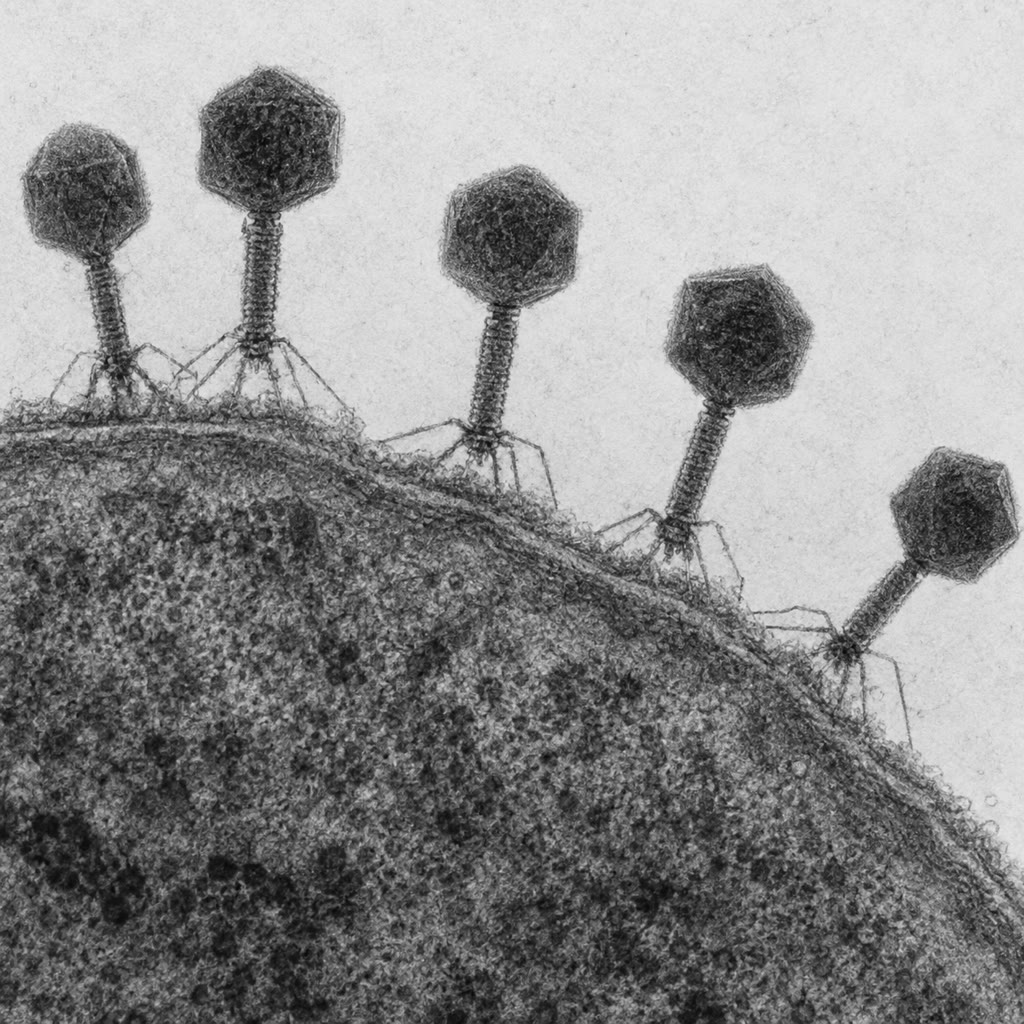
\includegraphics[width=0.36\linewidth]{images/book5/ai/b5-13-phage-tem.jpg}\hspace{0.04\linewidth}
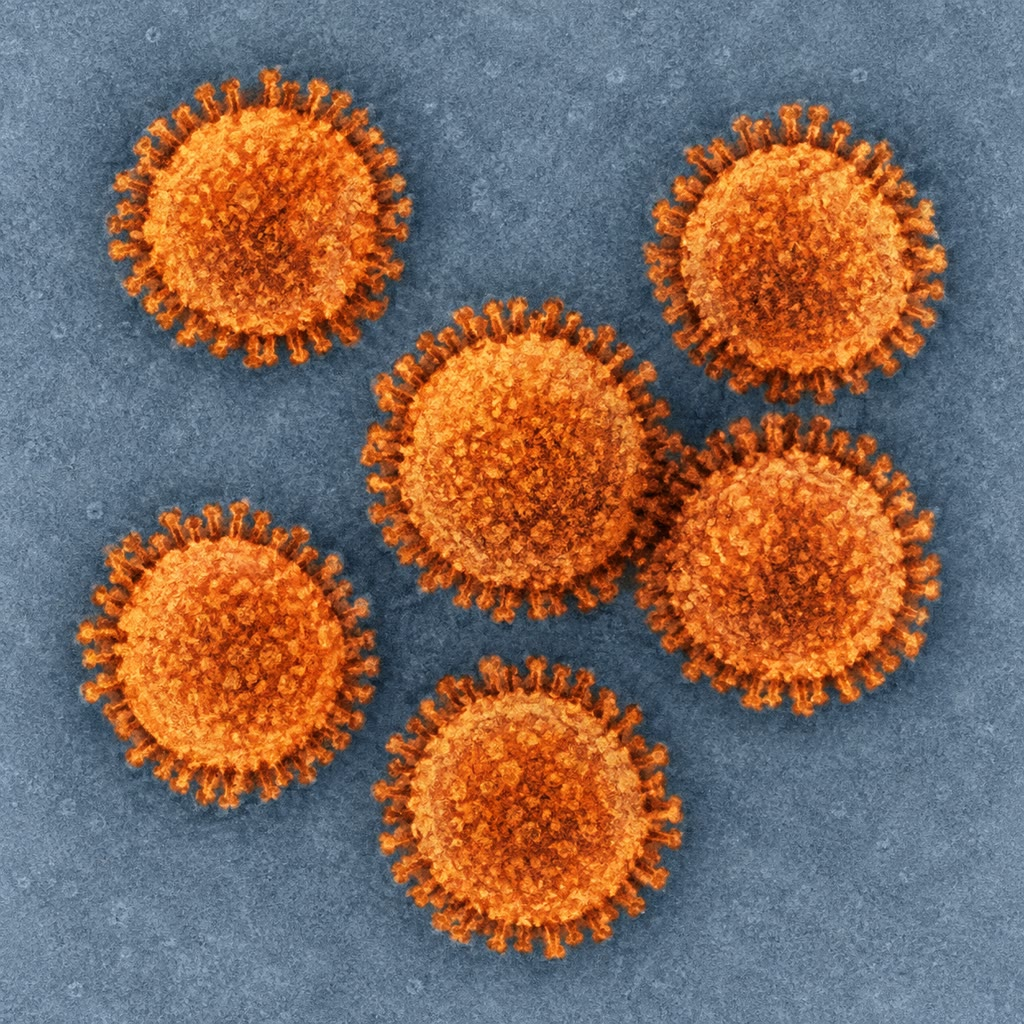
\includegraphics[width=0.36\linewidth]{images/book5/ai/b5-13-influenza-virions.jpg}

{\small يسارًا: عاثيات ملتصقة بألياف ذيولها ببكتيريا،
كل رأس منها \omterm{def:b3:virology:virus}{قفيصة} عشرينية من DNA. يمينًا: فيريونات
إنفلونزا مغلَّفة، وسطحها \omterm{def:b3:cytoskeleton-motility:cilia}{هدب} من أشواك الراصة الدموية و
النورامينيداز.}
\end{omfigure}

\section{كيف يتكاثر الفيروس}

\begin{definition}[دورة التضاعف]\label{def:b3:virology:cycle}
\index{دورة التضاعف الفيروسية}\index{مستقبل!فيروسي}\index{الاندماج اللايسوجيني}\index{الكمون}
يمر كل \omterm{def:b3:virology:virus}{فيروس} بالمراحل نفسها. \emph{الالتصاق} بمستقبل
مضيف بعينه --- CD4 ومستقبل كيموكين في HIV، وACE2
في فيروسات كورونا السارسية، وحمض السياليك في الإنفلونزا، و
\omterm{def:b3:bacteriology:envelope}{عديد سكريد شحمي} أو بورين في العاثية --- وهو يقرر أي
الأنواع وأي الخلايا يستطيع \omterm{def:b3:virology:virus}{الفيروس} أن يخمجها (وهو \emph{مداره}).
و\emph{الدخول}: اندماج \omterm{def:b3:virology:virus}{الغلاف} بالغشاء الهيولي، أو
التقام يتبعه اندماج من داخل \omterm{def:b3:membrane-traffic:endocytosis}{الجسيم الداخلي} الحمضي، أو، في
العاثية، حقن الجينوم عبر الجدار. و\emph{نزع \omterm{def:b3:virology:virus}{الغلاف}}، و
\emph{التعبير} عن المورّثات الفيروسية بالطريق الخاص بالصنف، و
\emph{تضاعف} الجينوم، في مصنع يبنيه \omterm{def:b3:virology:virus}{الفيروس} غالبًا
في الهيولى أو النواة. و\emph{التجميع}: تجميع قفيصات جديدة حول
جينومات جديدة، يقوده التجمع الذاتي للوحدات المتناظرة، و
\emph{الإطلاق}: إما بحلّ الخلية، وإما بالتبرعم عبر غشاء،
وهو ما يوفر \omterm{def:b3:virology:virus}{الغلاف}. وبعض الفيروسات يستطيع بدلًا من ذلك أن يقحم
جينومه في جينوم المضيف وينتظر: وهو \emph{الاندماج اللايسوجيني} في العاثية $\lambda$،
التي يبقيها كابحها صامتة حتى يتأذى المضيف؛ و
\emph{كمون} فيروسات الهربس في العصبونات مدى الحياة وكمون HIV
فيروسًا مندمجًا في الخلايا التائية الساكنة، ولا يزيله منها أي
دواء يعمل على التضاعف.
\end{definition}

\begin{omfigure}
\begin{tikzpicture}[every node/.style={font=\scriptsize}, >=stealth]
  % cell
  \draw[very thick, omDef, fill=omDef!6] (0,0) ellipse (5.6 and 3.2);
  \draw[thick, omDef!70, fill=omDef!20] (1.8,0) ellipse (1.6 and 1.1); \node at (1.8,0.75) {النواة};
  % virion outside
  \draw[thick, omProp, fill=omProp!30] (-7.2,1.6) circle (0.35); \foreach \a in {0,45,...,315} \draw[omProp, thick] (-7.2,1.6) ++(\a:0.35) -- ++(\a:0.15);
  \node[above] at (-7.2,2.1) {فيريون};
  \draw[->, thick] (-6.8,1.4) -- (-5.7,0.9); \node[below, align=center] at (-6.6,1.0) {1. الالتصاق\\بالمستقبل};
  % entry
  \draw[thick, omProp] (-5.4,0.7) arc[start angle=140, end angle=40, radius=0.5];
  \node[below, align=center] at (-3.9,-0.2) {2. الاندماج أو الالتقام؛\\3. نزع الغلاف};
  % genome path
  \draw[omThm, very thick] (-3.4,0.2) .. controls (-2.6,0.6) .. (-1.8,0.4);
  \draw[->, thick] (-1.6,0.4) -- (-0.4,0.4);
  \node[above, align=center] at (-1.0,0.55) {4. التعبير عن المورّثات،\\وتضاعف الجينوم};
  \draw[omThm, very thick] (-1.0,-0.5) -- (0.4,-0.5); \draw[omThm, very thick] (-1.0,-0.75) -- (0.4,-0.75); \draw[omThm, very thick] (-1.0,-1.0) -- (0.4,-1.0);
  % assembly
  \foreach \p in {(1.2,-1.6),(1.9,-1.9),(2.6,-1.5)} { \draw[thick, omProp, fill=omProp!30] \p circle (0.25); }
  \node[below, align=center] at (1.9,-2.2) {5. تجميع القفيصات\\حول الجينومات};
  % budding
  \draw[thick, omProp, fill=omProp!30] (4.9,-1.7) circle (0.32); \draw[->, thick] (5.3,-1.75) -- (6.4,-2.0);
  \draw[thick, omProp, fill=omProp!30] (7.0,-2.2) circle (0.35); \foreach \a in {0,45,...,315} \draw[omProp, thick] (7.0,-2.2) ++(\a:0.35) -- ++(\a:0.15);
  \node[below, align=center] at (6.4,-2.6) {6. التبرعم عبر الغشاء\\(الغلاف) أو حلّ الخلية};
  % latency
  \draw[->, thick, dashed, omMeth!70!black] (-0.2,0.2) -- (0.9,0.2); \node[below, omMeth!70!black, align=center, font=\tiny] at (2.0,-0.05) {الفيروسات الرجعية: تندمج\\فيروسًا مندمجًا؛ الكمون};
\end{tikzpicture}

{\small دورة تضاعف \omterm{def:b3:virology:virus}{فيروس} مغلَّف: الالتصاق بمستقبل،
والدخول ونزع \omterm{def:b3:virology:virus}{الغلاف}، والتعبير والتضاعف في آلة
المضيف، والتجميع، والإطلاق بالتبرعم --- أو، في \omterm{def:b3:virology:virus}{الفيروس} الرجعي،
الاندماج في جينوم المضيف والصمت.}
\end{omfigure}

\begin{method}[عدّ الجسيمات المعدية: مقايسة اللويحات]\label{met:b3:virology:plaque}
\index{مقايسة اللويحات}\index{العيار}
لقياس مخزون فيروسي: (1) مدّده بخطوات عشرية؛ (2) اخلط كل
تمديد بفائض من الخلايا المضيفة --- بكتيريا في أغار لين
للعاثية، وطبقة أحادية من خلايا مزروعة \omterm{def:b3:virology:virus}{لفيروس} حيواني؛ (3) حضّن:
فيخمج كل جسيم معدٍ خلية واحدة، وتخمج الذرية
الجيران، وبعد يوم أو يومين تعلّم الموضعَ ثقبةٌ صافية هي
\emph{اللويحة}؛ (4) عُدّ اللويحات على طبق فيه \numrange{30}{300}
واضرب في التمديد: فينتج \emph{العيار} بوحدات تكوين اللويحات
(PFU) في المليلتر. ولأن كل لويحة نسيلة من جسيم واحد،
فالتقاطها يعطي عزلة نقية. ونسبة الجسيمات الفيزيائية
(المعدودة بالمجهر الإلكتروني أو بتفاعل PCR) إلى وحدات تكوين اللويحات
أعلى من واحد بكثير عادةً --- من عشرة إلى ألف في كثير من الفيروسات الحيوانية ---
لأن معظم الجسيمات معطوبة أو تخفق في الإخماج.
\end{method}

\begin{omfigure}
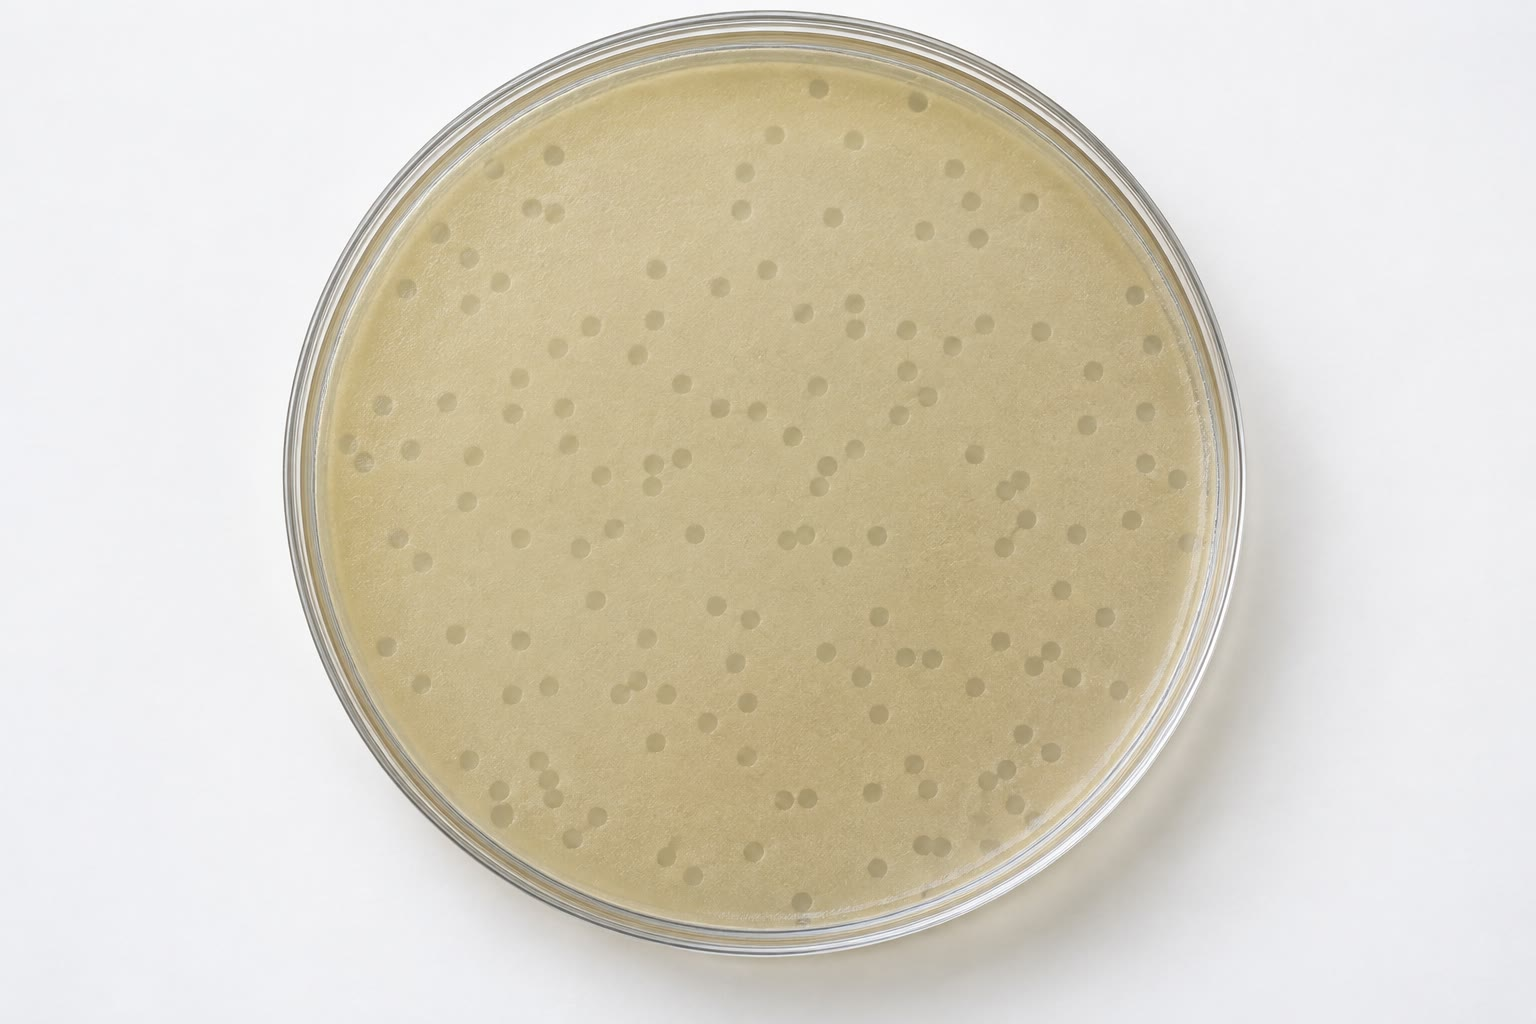
\includegraphics[width=0.46\linewidth]{images/book5/ai/b5-13-plaque-assay.jpg}\hspace{0.04\linewidth}
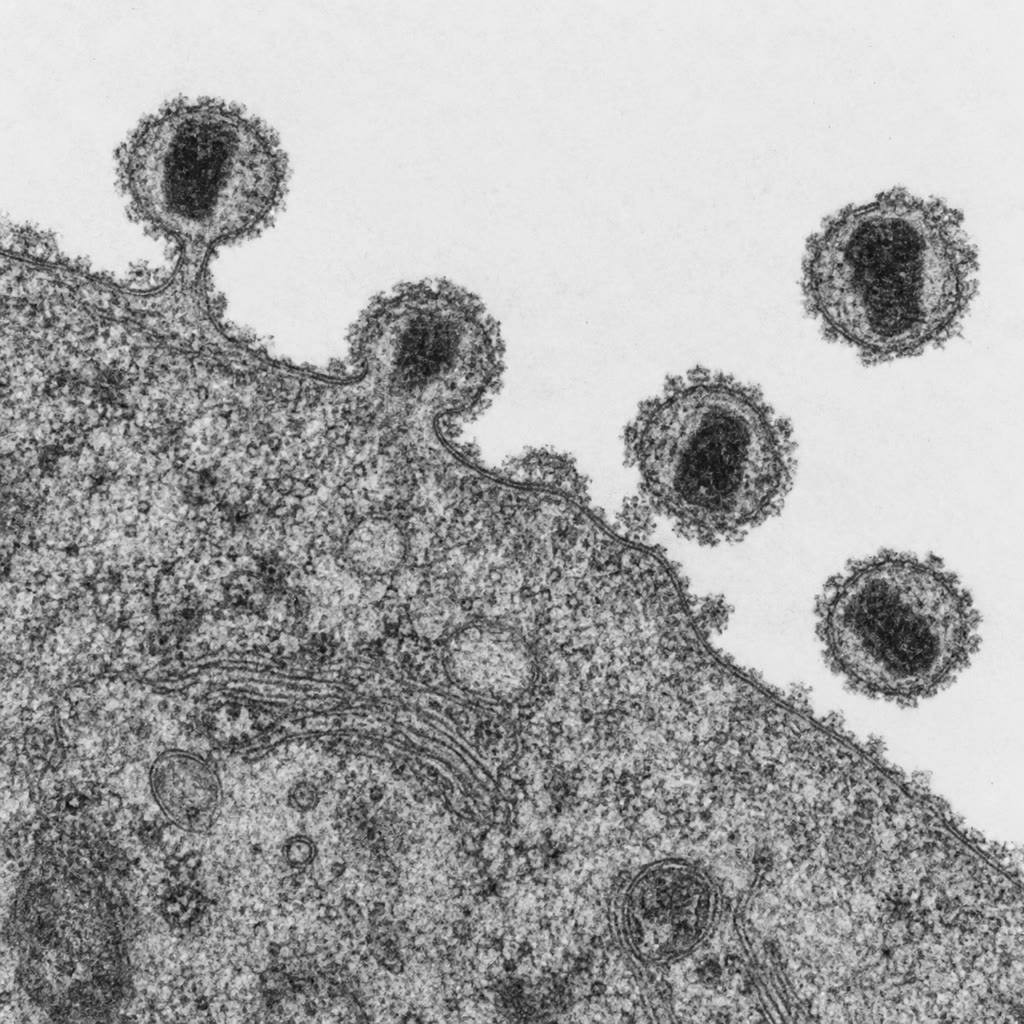
\includegraphics[width=0.36\linewidth]{images/book5/ai/b5-13-hiv-budding.jpg}

{\small يسارًا: لويحات في بساط بكتيري، كل منها منطقة صافية حلّت
فيها ذرية عاثية واحدة الخلايا حولها. يمينًا: جسيمات HIV
تتبرعم من لمفاوية تائية، آخذةً غلافها من
غشاء الخلية.}
\end{omfigure}

\begin{theorem}[حركية الخمج داخل المضيف]\label{thm:b3:virology:dynamics}
\index{عدد التكاثر الأساسي!داخل المضيف}\index{الحمل الفيروسي}\index{حركية الفيروس}
لتكن $T$ كثافة الخلايا الهدف القابلة، و$I$ كثافة الخلايا المخموجة
و$V$ كثافة الفيريونات الحرة. وتخمج الفيريونات الأهداف بمعدل $\beta TV$،
وتنتج الخلايا المخموجة فيريونات بمعدل $p$ لكل منها وتموت بمعدل
$\delta$، وتُصفّى الفيريونات الحرة بمعدل $c$:
\[
\frac{\mathrm{d}I}{\mathrm{d}t} = \beta TV - \delta I, \qquad
\frac{\mathrm{d}V}{\mathrm{d}t} = pI - cV .
\]
وبإبقاء $T$ ثابتة، ينمو الخمج إذا تجاوز \emph{عدد التكاثر
الأساسي} $R_{0} = \beta Tp/(c\delta)$ القيمةَ $1$، وعند
الحالة المستقرة $V^{*} = p I^{*}/c$ مع توازن الإنتاج والتصفية.
وإذا أوقف دواء كل خمج جديد عند $t = 0$ ($\beta \to 0$)، تلاشت
الفيريونات أولًا بمعدل التصفية $c$، ثم، متى هبط \omterm{def:b3:virology:virus}{الفيروس}
الحر إلى المستوى الذي تبقيه الخلايا المخموجة الباقية، بمعدل
موت تلك الخلايا $\delta$:
\[
V(t) \approx V_{0}\,\frac{c\,e^{-\delta t} - \delta\,e^{-ct}}{c - \delta}
\;\longrightarrow\; V_{0}\,\frac{c}{c-\delta}\,e^{-\delta t}
\quad (t \gg 1/c).
\]
وميلا \omterm{thm:b3:virology:dynamics}{الحمل الفيروسي} بعد العلاج يقيسان $c$ و
$\delta$، ويعطي $pI^{*} = cV^{*}$ الإنتاج اليومي للفيريونات
قبل العلاج.
\end{theorem}
\begin{proof}
تعيش الخلية المخموجة وسطيًا $1/\delta$ وتصنع $p/\delta$
فيريونًا؛ ويعيش كل \omterm{def:b3:virology:virus}{فيريون} $1/c$ ويخمج $\beta T/c$ خلية في ذلك
الزمن؛ وجداؤهما عدد الخلايا المخموجة التي تنشأ عن خلية مخموجة
واحدة، وهو $R_{0}$. وعند الحالة المستقرة يعطي $\mathrm{d}V/\mathrm{d}t = 0$
القيمةَ $V^{*} = pI^{*}/c$. وبعد العلاج تكون $\mathrm{d}I/\mathrm{d}t =
-\delta I$، ومنه $I = I_{0}e^{-\delta t}$، وتكون $\mathrm{d}V/\mathrm{d}t =
pI_{0}e^{-\delta t} - cV$ معادلة خطية حلها عند
$V(0) = V_{0} = pI_{0}/c$ هو العبارة المعطاة (وللتحقق: عند $t = 0$
تساوي $V_{0}$، وهي تحقق المعادلة حدًا حدًا). ومن أجل $t
\gg 1/c$ يزول الحد $e^{-ct}$ وتتبع $V$ الخلايا المخموجة
بميل $-\delta$؛ ومن أجل $t \ll 1/\delta$ و$c \gg \delta$ يكون الميل
الباكر $-c$.
\end{proof}

\begin{example}[HIV قبل المعادلات وبعدها]\label{ex:b3:virology:hiv}
حتى عام 1995 كانت سنوات \omterm{def:b3:virology:cycle}{الكمون} السريري في خمج HIV --- أي حمل
فيروسي ثابت قدره $10^{4}$--$10^{6}$ نسخة في المليلتر وهبوط بطيء في
الخلايا التائية --- تُقرأ فيروسًا هادئًا. فأعطى هو وبيرلسون وزملاؤهما
المرضى \omterm{def:b3:virology:drugs}{مثبط بروتياز} وطابقوا هبوط \omterm{thm:b3:virology:dynamics}{الحمل
الفيروسي} على المبرهنة: فأعطى الطور السريع $c \approx \qty{3}{d^{-1}}$
(أي عمر نصف \omterm{def:b3:virology:virus}{للفيريون} قدره نحو ست ساعات)، وأعطى الطور البطيء $\delta \approx
\qty{0.5}{d^{-1}}$ (فتعيش الخلية المخموجة نحو يوم ونصف). و
الحمل الثابت البالغ $10^{5}$ في المليلتر في \qty{15}{L} من سوائل الجسم،
المصفّى بمعدل $c$، يقتضي إذن إنتاج نحو $10^{10}$
\omterm{def:b3:virology:virus}{فيريون} في اليوم، كل يوم، سنين: فالفترة ``الكامنة''
حالة مستقرة محمومة من الخمج والموت، ومخزون الخلايا التائية
يُستبدل يوميًا حتى يخفق. ويتبع حساب الطفرات في القسم
التالي فورًا، ومعه سبب إخفاق الأدوية المفردة
ونجاح الثلاثة.
\end{example}

\begin{omfigure}
\begin{tikzpicture}
\begin{axis}[
  width=0.7\linewidth, height=5.8cm,
  axis x line=bottom, axis y line=left,
  xmin=0, xmax=14, ymin=10, ymax=2e5, ymode=log,
  xlabel={الأيام بعد بدء العلاج}, ylabel={فيريونات في المليلتر},
  xlabel style={font=\small, at={(axis description cs:0.5,-0.12)}, anchor=north}, ylabel style={font=\small},
  tick label style={font=\small}, xtick={0,2,4,6,8,10,12,14},
  clip=false,
]
\addplot[very thick, omDef, domain=0:14, samples=100] {1e5*(3*exp(-0.5*x) - 0.5*exp(-3*x))/2.5};
\addplot[dashed, omThm, domain=0:1.6, samples=2] {1e5*exp(-3*x)};
\addplot[dashed, omMeth!70!black, domain=1.5:14, samples=2] {1e5*1.2*exp(-0.5*x)};
\node[font=\scriptsize, omThm, anchor=west] at (axis cs:1.8,600) {تصفية الفيريونات الحرة: ميل $-c$، وعمر نصف \qty{6}{h}};
\node[font=\scriptsize, omMeth!70!black, anchor=south west] at (axis cs:5.5,1.5e4) {موت الخلايا المخموجة: ميل $-\delta$، وعمر نصف \qty{1.4}{d}};
\end{axis}
\end{tikzpicture}

{\small \omterm{thm:b3:virology:dynamics}{الحمل الفيروسي} بعد أن يوقف دواء الأخماج الجديدة، من المبرهنة
عند $c = \qty{3}{d^{-1}}$ و$\delta = \qty{0.5}{d^{-1}}$: هبوط سريع
مع تصفية الفيريونات الحرة، ثم هبوط أبطأ يوقّته موت
الخلايا المخموجة سلفًا.}
\end{omfigure}

\section{كيف تتطور الفيروسات}

\begin{definition}[الطفرة، وشبه النوع، والانجراف والإزاحة]\label{def:b3:virology:evolution}
\index{شبه النوع}\index{انجراف مستضدي}\index{إزاحة مستضدية}\index{إعادة التوزيع}
البوليميرازات المعتمدة على RNA والناسخات العكسية لا تدقيق
لها، وتطفر فيروسات RNA بمعدل $10^{-4}$ إلى $10^{-6}$ لكل
نوكليوتيد في كل تضاعف --- أي ألف إلى مليون ضعف معدل
مضيفاتها --- فتكون جمهرة \omterm{def:b3:virology:virus}{فيروس} RNA سحابة من
الجينومات القريبة، هي \emph{شبه النوع}، يحضر فيها كل طافر نقطي
مفرد في كل حين إذا كانت الجمهرة كبيرة. والانتقاء
بالأجسام المضادة يقود \emph{الانجراف المستضدي}: فبروتينات سطح
الإنفلونزا تتراكم فيها التبديلات سنةً بعد سنة، و
تحمي مناعة العام الماضي أقل في كل موسم. أما \emph{الإزاحة المستضدية} فقفزة: إذ
يمكن \emph{إعادة توزيع} جينوم مجزأ (وللإنفلونزا ثماني قطع من RNA)
حين تخمج سلالتان خلية واحدة، والقطعة التي
تشفّر راصة دموية من \omterm{def:b3:virology:virus}{فيروس} طير أو خنزير، ولا مناعة لأي إنسان
تجاهها، تنتج جائحة --- في 1918 و1957 و1968 و2009.
وإعادة التركيب داخل جينوم تفعل الشيء نفسه في الفيروسات غير المجزأة،
وفيروسات كورونا تعيد التركيب بحرية. ومعظم الفيروسات البشرية الجديدة
\emph{أمراض حيوانية المصدر}، تعبر من مستودع حيواني --- الخفافيش لفيروسات
كورونا والإيبولا والكلَب؛ والطيور والخنازير للإنفلونزا؛ والرئيسيات
\omterm{def:b3:virology:virus}{لفيروس} HIV --- والعبور مسألةُ بضع طفرات في
بروتين رابط لمستقبل عادةً.
\end{definition}

\begin{proposition}[عتبة الخطأ]\label{prop:b3:virology:error-threshold}
\index{عتبة الخطأ}\index{تدقيق!فيروسي}
جينوم من $L$ نوكليوتيد يُنسخ بمعدل خطأ $u$ لكل نوكليوتيد
يُنسخ بلا أي خطأ باحتمال $(1-u)^{L} \approx e^{-uL}$.
ولكي يدوم التسلسل الأصلح في الجمهرة في مواجهة
طوفان طافراته، يجب أن تتجاوز نسبة النسخ الخالية من الخطأ
نحو مقلوب أفضليته الانتقائية $\sigma$: أي $e^{-uL} \gtrsim
1/\sigma$، وهذا يعني $uL \lesssim \ln\sigma$، وهو عدد من رتبة الواحد. و
جداء معدل الطفرة في طول الجينوم محدود إذن: \omterm{def:b3:virology:virus}{ففيروس}
RNA عند $u = 10^{-4}$ لا يمكن أن يكون جينومه أطول بكثير من
$10^{4}$ نوكليوتيد، وهو نحو ما لفيروسات RNA، و
فيروسات كورونا، وجينوماتها البالغة \qty{30}{kb} أطول جينومات RNA المعروفة، لا تبلغه
إلا بتشفير نوكلياز خارجي مدقِّق يخفض $u$ عشرة أضعاف. و
العتبة سلاح أيضًا: فالأدوية التي ترفع معدل خطأ البوليميراز
(الريبافيرين، والمولنوبيرافير) تدفع فيروسًا فوقها إلى \emph{كارثة
الخطأ}، فينهار \omterm{def:b3:virology:evolution}{شبه النوع}.
\end{proposition}
\begin{proof}
تعطي الأخطاء المستقلة عند كل موضع من المواضع $L$ احتمال الخلو من الخطأ
$(1-u)^{L}$، و$\ln(1-u) \approx -u$ من أجل $u$ صغيرة. وتوازن
الجمهرة هو حجة \omterm{def:b3:virology:evolution}{شبه النوع} المعيارية (آيغن، 1971): فالتسلسل
السيد يُجدَّد بمعدل $\sigma e^{-uL}$ نسبةً إلى الطافر
الوسطي ويُفقد إلى الطفرة فيما عدا ذلك؛ ولا يُصان إلا إذا تجاوز
الأولُ العددَ $1$، ومنه الحد.
\end{proof}

\begin{omfigure}
\begin{tikzpicture}[every node/.style={font=\scriptsize}, >=stealth]
  % drift
  \begin{scope}
    \foreach \i in {0,1,2,3} { \draw[thick, omProp, fill=omProp!30] (\i*1.3,0) circle (0.35); \foreach \a in {0,60,...,300} \draw[omProp, thick] (\i*1.3,0) ++(\a:0.35) -- ++(\a:0.14); }
    \foreach \i/\n in {1/1,2/2,3/3} { \foreach \k in {1,...,\n} \fill[omThm] (\i*1.3,0) ++({60*\k+20}:0.5) circle (0.06); }
    \foreach \i in {0,1,2} \draw[->, thick] (\i*1.3+0.5,0) -- (\i*1.3+0.8,0);
    \node[below, align=center] at (1.95,-0.6) {الانجراف المستضدي: تتراكم الطفرات النقطية\\في بروتينات السطح، موسمًا بعد موسم};
  \end{scope}
  % shift
  \begin{scope}[xshift=7.0cm]
    \draw[thick, omProp, fill=omProp!30] (0,0.5) circle (0.4); \foreach \y in {-0.2,-0.1,0,0.1,0.2} \draw[omProp!80!black] (-0.25,0.5+\y) -- (0.25,0.5+\y);
    \draw[thick, omMeth!70!black, fill=omMeth!30] (0,-0.7) circle (0.4); \foreach \y in {-0.2,-0.1,0,0.1,0.2} \draw[omMeth!70!black] (-0.25,-0.7+\y) -- (0.25,-0.7+\y);
    \node[left, align=right] at (-0.5,0.5) {سلالة بشرية،\\8 قطع}; \node[left, align=right] at (-0.5,-0.7) {سلالة طير،\\8 قطع};
    \draw[->, thick] (0.5,0.4) -- (1.5,0.0); \draw[->, thick] (0.5,-0.6) -- (1.5,-0.2);
    \draw[thick, omDef, fill=omDef!10] (2.4,-0.1) ellipse (0.9 and 0.7); \node[below] at (2.4,-0.85) {خلية واحدة (في خنزير)};
    \draw[->, thick] (3.4,-0.1) -- (4.3,-0.1);
    \draw[thick, omProp, fill=omProp!30] (4.9,-0.1) circle (0.4); \foreach \y in {-0.2,-0.1,0.1,0.2} \draw[omProp!80!black] (4.65,-0.1+\y) -- (5.15,-0.1+\y); \draw[omMeth!70!black, very thick] (4.65,-0.1) -- (5.15,-0.1);
    \node[right, align=left] at (5.4,-0.1) {معاد التوزيع: راصة\\دموية طير في\\فيروس بشري};
    \node[below, align=center] at (2.4,-1.5) {الإزاحة المستضدية: تُبادَل قطع كاملة؛\\ولا أحد ممنّع --- أي جائحة};
  \end{scope}
\end{tikzpicture}

{\small طريقان يفلت بهما \omterm{def:b3:virology:virus}{فيروس} الإنفلونزا من المناعة. الانجراف: تتراكم الطفرات
في الأشواك تدريجيًا. والإزاحة: سلالتان في خلية واحدة تتبادلان
قطع جينوم كاملة، فيظهر بروتين شوكة جديد على البشر
دفعةً واحدة.}
\end{omfigure}

\begin{example}[لماذا احتاج HIV إلى ثلاثة أدوية]\label{ex:b3:virology:three-drugs}
تخطئ ناسخة HIV العكسية نحو مرة في $10^{5}$ نوكليوتيد، فيحمل
كل جينوم من \qty{9700}{nt} يُنسخ نحو $0.1$ طفرة، و
$10^{10}$ جينوم جديد في اليوم تحمل $10^{9}$ طفرة بينها: فكل
واحدة من الطفرات النقطية المفردة الممكنة البالغة $3\times 9700 \approx \num{30000}$
تنشأ مرات كثيرة كل يوم، قبل إعطاء أي دواء. و
الدواء الذي تهزمه طفرة واحدة --- كما تهزم طفرة واحدة معظم
مثبطات الناسخة العكسية والبروتياز --- يُهزم إذن
في أسابيع، وهو ما حدث لدواء AZT عام 1987. أما الطفرتان المستقلتان
فتنشآن معًا بمعدل $10^{-10}$ لكل جينوم، أي نحو مرة في اليوم؛
والثلاث عند $10^{-15}$، أي مرة في ألف يوم --- والمريض على ثلاثة
أدوية هبط حمله ألف ضعف ينتج $10^{7}$ جينوم في
اليوم، فلا يظهر الطافر الثلاثي قط. وذلك، مع
برهان المبرهنة على أن \omterm{def:b3:virology:virus}{الفيروس} كان يتضاعف بأقصى سرعته، جعل
\omterm{thm:b3:cancer-biology:goldie-coldman}{المعالجة التوليفية} منذ عام 1996 العلاجَ الذي حوّل الإيدز إلى
حالة مزمنة.
\end{example}

\section{المضيفات والدفاعات والأدوية}

\begin{proposition}[الإمراض والدفاع]\label{prop:b3:virology:pathogenesis}
\index{أثر اعتلالي خلوي}\index{إنترفيرون}\index{القطع!في العاثيات}
يضر \omterm{def:b3:virology:virus}{الفيروس} بحلّ الخلايا (فشلل الأطفال يهدم العصبونات الحركية، وHIV يقتل
الخلايا التائية)، وبجعل الخلايا تنتج نواتج سامة، وبتحويلها
(\cref{ch:b3:cancer-biology})، وغالبًا أساسًا عبر استجابة
المضيف نفسه: الحمى، وأذية الأنسجة، وفي أسوأ الأحوال عاصفة السيتوكينات في
التفاعل المناعي تجاه الإنفلونزا أو فيروسات كورونا السارسية. ويجيب المضيف
بدفاعات فطرية تتعرف بصمات التضاعف
الفيروسي --- RNA مزدوج الطاق، وRNA بلا قلنسوة، وDNA في
العصارة --- وترد بمادة \emph{الإنترفيرون}، الذي يضع كل
خلية مجاورة في حالة مضادة للفيروسات (\cref{ch:b3:innate-immunity})؛
وبخلايا قاتلة طبيعية تهدم الخلايا التي أخفت MHC عندها؛
وبأجسام مضادة تعادل الفيريونات وخلايا تائية سامة تقتل
الخلايا المخموجة قبل أن تطلق ذريتها (\cref{ch:b3:adaptive-immunity})؛
وفي البكتيريا بإنزيمات قطع تقطع DNA الغريب وبذاكرة
\omterm{def:b3:genetic-engineering:crispr}{CRISPR} في \cref{ch:b3:genetic-engineering}. وترد الفيروسات:
فيكاد كل \omterm{def:b3:virology:virus}{فيروس} كبير يشفّر بروتينات تحجب الإنترفيرون، أو تخفي
MHC، أو تحاكي السيتوكينات أو تثبط \omterm{def:b3:cell-cycle-apoptosis:apoptosis}{الاستماتة}، وسباق التسلح
مكتوب في الجينومين معًا.
\end{proposition}

\begin{definition}[الأدوية المضادة للفيروسات واللقاحات]\label{def:b3:virology:drugs}
\index{دواء مضاد للفيروسات}\index{نظير نوكليوزيد}\index{مثبط بروتياز}\index{لقاح}\index{لقاح mRNA}
تهاجم الأدوية المضادة للفيروسات الإنزيمات الفيروسية أو الخطوات التي لا تنفذها
الخلية المضيفة. و\emph{نظائر النوكليوزيد} منهيات سلسلة: فالأسيكلوفير
لا يفسفره إلا كيناز الثيميدين في \omterm{def:b3:virology:virus}{فيروس} الهربس ثم
يحجب بوليميراز DNA الفيروسي، فلا يعمل إلا في الخلايا المخموجة؛
وAZT والتينوفوفير واللاميفودين توقف الناسخة العكسية؛ والريمديسيفير و
المولنوبيرافير يعملان على بوليميراز \omterm{def:b3:virology:virus}{فيروس} كورونا، والثاني
بالتطفير. و\emph{مثبطات البروتياز} تحجب شطر متعددات الببتيد
الفيروسية (في HIV، والتهاب الكبد C، والنيرماتريلفير ضد SARS-CoV-2). ومثبطات
الإنتغراز توقف تكوّن \omterm{def:b3:virology:virus}{فيروس} HIV المندمج؛ ومثبطات النورامينيداز توقف
انفصال فيريونات الإنفلونزا عن الخلية التي تتبرعم منها؛ ومثبطات
الدخول تحجب مستقبلًا. ويُشفى \omterm{def:b3:virology:virus}{فيروس} التهاب الكبد C اليوم في
اثني عشر أسبوعًا بتوليفات من أدوية مباشرة الفعل، وهو أول خمج
فيروسي مزمن يُشفى بالمعالجة الكيميائية. و\emph{اللقاحات} تعرض
مستضدات \omterm{def:b3:virology:virus}{الفيروس} بلا مرضه: \omterm{def:b3:virology:virus}{فيروس} حي موهَّن (الحصبة، و
شلل الأطفال بالفم، والحمى الصفراء)، أو \omterm{def:b3:virology:virus}{فيروس} معطَّل (شلل الأطفال بالحقن، و
الإنفلونزا)، أو وحدة فرعية (مستضد سطح التهاب الكبد B المصنوع في الخميرة، و
بروتين \omterm{def:b3:virology:virus}{قفيصة} \omterm{def:b3:virology:virus}{فيروس} \omterm{def:b3:cancer-biology:hallmarks}{الورم} الحليمي)، أو ناقل فيروسي غير ضار يحمل
مورّثة الهدف، أو، منذ عام 2020، \emph{RNA الرسول} المشفِّر
للمستضد، موصلًا في جسيمات نانوية دهنية، تترجمه خلايا
المتلقي نفسه. وأما مناعيًا لماذا تنجح، وكم يجب أن يُلقَّح
لحماية الباقين، فذلك موضوع
\cref{ch:b3:adaptive-immunity}.
\end{definition}

\begin{remark}[الفيروسات في اقتصاد الحياة]\label{rem:b3:virology:economy}
الفيروسات التي تضر البشر خطأ تقريب في جمهرة فيروسات
العالم، ومعظمها يخمج البكتيريا والعتائق. والعاثيات تقتل
خُمس بكتيريا المحيط إلى ثلثها يوميًا وتعيد
محتوياتها إلى المخزون الذائب --- وهو \emph{المحوّل الفيروسي} في
دورة الكربون في كتاب السنة~الثانية. وهي تنقل المورّثات بين البكتيريا
(\cref{ch:b3:bacteriology})، وذيفاناتها هي ذيفانات
الخناق والكوليرا وأسوأ سلالات \emph{E.~coli}. وثمانية في المئة من
الجينوم البشري بقايا فيروسات رجعية قديمة
(\cref{ch:b3:genomics})، وإحدى مورّثات غلافها تلحم اليوم
خلايا المشيمة. فالفيروسات أكبر مخزون للجدة
الوراثية على الكوكب، وحدُّ ما يُعدّ حيًا يمر
خلالها.
\end{remark}

\section{تمارين}

\begin{exercise}[$\star$]\label{exo:b3:virology:1}
ضع شلل الأطفال والإنفلونزا وHIV والهربس البسيط والتهاب الكبد B \omterm{def:b3:virology:virus}{والفيروس} العجلي
في أصنافها البالتيمورية وقل أي إنزيم يجب أن يجلبه أو يصنعه كل منها
مما تخلو منه الخلية.
\end{exercise}

\begin{exercise}[$\star$]\label{exo:b3:virology:2}
ماذا بيّنت تجربة هيرشي وتشيس، وماذا كان ليُوجد
لو كان البروتين يحمل التعليمات؟
\end{exercise}

\begin{exercise}[$\star$]\label{exo:b3:virology:3}
مخزون عاثية ممدَّد $10^{-7}$ يعطي $84$ لويحة من \qty{0.1}{mL}.
فما العيار؟ ولماذا قد يعدّ المجهر الإلكتروني عشرة أضعاف
الجسيمات؟
\end{exercise}

\begin{exercise}[$\star$]\label{exo:b3:virology:4}
عدّد مراحل دورة التضاعف الست وسمِّ لكل منها دواءً
مضادًا للفيروسات أو دفاعًا مضيفًا يعمل عليها.
\end{exercise}

\begin{exercise}[$\star\star$]\label{exo:b3:virology:5}
باستعمال \cref{prop:b3:virology:economy}، احسب الحمض النووي اللازم
لتشفير \omterm{def:b3:virology:virus}{قفيصة} \omterm{def:b3:virology:virus}{فيروس} مصنوعة من $180$ نسخة من بروتين
كتلته \qty{30}{kDa}، وقارنه بجينوم قدره \qty{4.5}{kb} قد يكون \omterm{def:b3:virology:virus}{لفيروس}
كهذا. وما نسبة مورّثة \omterm{def:b3:virology:virus}{القفيصة} من الجينوم؟
\end{exercise}

\begin{exercise}[$\star\star$]\label{exo:b3:virology:6}
عند $c = \qty{3}{d^{-1}}$ و$\delta = \qty{0.5}{d^{-1}}$ و$V_{0} =
10^{5}$ في المليلتر، احسب $V$ من المبرهنة عند $t = 0.5$ و$2$ و
$10$ أيام. وكم يمضي حتى يهبط الحمل دون $50$ في المليلتر، وهو حد
الكشف؟
\end{exercise}

\begin{exercise}[$\star\star$]\label{exo:b3:virology:7}
\omterm{def:b3:virology:virus}{فيروس} RNA عنده $u = 3\times 10^{-5}$ و$L = \qty{12}{kb}$. فما
نسبة جينومات ذريته التي لا تحمل طفرة؟ وماذا يحدث لتلك
النسبة إذا رفع دواء مطفِّر $u$ ثلاثة أضعاف؟ وفسّر لماذا احتاجت
فيروسات كورونا إلى إنزيم مدقِّق.
\end{exercise}

\begin{exercise}[$\star\star$]\label{exo:b3:virology:8}
فسّر الانجراف والإزاحة المستضديين في الإنفلونزا، ولماذا حملت
السلالة الجائحية حتى الآن راصة دموية جديدة دائمًا.
\end{exercise}

\begin{exercise}[$\star\star$]\label{exo:b3:virology:9}
الأسيكلوفير نظير غوانوزين يجب أن يُفسفر ليعمل.
فسّر لماذا يضر الخلايا المخموجة بالهربس دون غيرها، وتنبأ
بطفرات المقاومة.
\end{exercise}

\begin{exercise}[$\star\star\star$]\label{exo:b3:virology:10}
اشتق $R_{0} = \beta Tp/(c\delta)$ من معادلتي
المبرهنة بإيجاد شرط نمو خمج صغير ($I$ و$V$ قرب
الصفر، و$T$ ثابتة)، وفسّر كل عامل.
\end{exercise}

\begin{exercise}[$\star\star\star$]\label{exo:b3:virology:11}
مريض على علاج فعال ما يزال يؤوي $10^{6}$ خلية تائية ساكنة
مخموجة كمونيًا فيروسها المندمج صامت، وعمر نصفها
$44$ شهرًا. فكم يجب أن يستمر العلاج ليهبط المستودع
دون خلية واحدة؟ ولماذا يجعل هذا HIV غير قابل للشفاء بأدوية
تحجب التضاعف، وماذا يقتضي الشفاء؟
\end{exercise}

\begin{exercise}[$\star\star\star$]\label{exo:b3:virology:12}
فسّر حجة \cref{ex:b3:virology:three-drugs} بأرقامك أنت
\omterm{def:b3:virology:virus}{لفيروس} قدره \qty{30}{kb} عند $u = 10^{-6}$ ينتج $10^{9}$
جينوم في اليوم. فكم دواءً تركّب، ولماذا قد لا تُعدّ أدوية
ضد موقعين من الإنزيم نفسه دواءين؟
\end{exercise}

\section{مسألة: فيروس في مريض}

\begin{problem}[{مسألة نهاية الأسبوع --- خمج HIV معدودًا فيريونًا
فيريونًا، وحركيته مطابَقة لمنحني علاج، وطفراته محسوبة
في مواجهة الأدوية، ومستودعه موقوتًا، وتنتهي إلى الإنتاج
اليومي للفيريونات، واليوم الذي يصير فيه الحمل غير مكشوف و
احتمال وجود طافر ثلاثي}]
\label{pb:b3:virology:1}
معطيات: \omterm{thm:b3:virology:dynamics}{الحمل الفيروسي} $V^{*} = 2\times 10^{5}$ في المليلتر في \qty{15}{L} من سوائل
الجسم؛ و$c = \qty{3}{d^{-1}}$، و$\delta = \qty{0.5}{d^{-1}}$؛ وتصنع كل خلية
مخموجة $p = 500$ \omterm{def:b3:virology:virus}{فيريون} في اليوم؛ والجينوم \qty{9700}{nt}، و$u = 10^{-5}$
لكل نوكليوتيد في التضاعف؛ وطفرات مفردة تمنح مقاومةً
لكل من ثلاثة أدوية؛ وعلى المعالجة الثلاثية يهبط الإنتاج إلى $10^{7}$
جينوم في اليوم؛ والمستودع الكامن $10^{6}$ خلية، عمر نصفها $44$ شهرًا؛
\omterm{def:b3:virology:virus}{والفيريون} كرة قطرها \qty{120}{nm} تحوي طاقي RNA من \qty{9700}{nt}
ونحو \num{2000} جزيء بروتين كتلة كل منها \qty{25}{kDa}.

\medskip
\noindent\textbf{الجزء الأول --- العدّ.}
\begin{enumerate}
  \item كم فيريونًا في الجسم عند الحالة المستقرة؟
  \item كم يُصفّى في اليوم، ومن ثم كم يُنتج في اليوم؟
  \item كم خلية مخموجة تنتجها، وكم يموت منها في
        اليوم؟
  \item ما كتلة \omterm{def:b3:virology:virus}{الفيريون} الواحد (مع RNA عند \qty{330}{Da} لكل
        نوكليوتيد زائدًا البروتين)، وما الكتلة الكلية للفيريونات في
        الجسم؟ قارنها بحبة رمل (\qty{1}{mg}).
  \item في الجسم $10^{12}$ خلية تائية CD4 ويستبدل المخموجة
        منها. فما نسبة المخزون المخموجة في أي لحظة، و
        كيف تقتل نسبة بهذا الصغر المخزونَ في عشر سنوات؟
  \item إذا ماتت كل خلية مخموجة \omterm{def:b3:cell-cycle-apoptosis:apoptosis}{بالاستماتة} وابتُلعت في غضون
        ساعة (\cref{ch:b3:cell-cycle-apoptosis})، فكم منها تُصفّى
        في أي لحظة؟
\end{enumerate}

\medskip
\noindent\textbf{الجزء الثاني --- العلاج.}
\begin{enumerate}[resume]
  \item يوقف العلاج الأخماج الجديدة عند $t = 0$. احسب $V$ عند $t =
        1$ و$3$ و$7$ و$14$ يومًا من المبرهنة.
  \item في أي يوم يهبط الحمل دون حد الكشف البالغ
        $50$ في المليلتر؟
  \item من الميلين، كيف يقدّر الطبيب $c$ و
        $\delta$ من قياسات في الأيام $0$--$1$ و$3$--$10$؟
  \item بعد الطورين يستوي الحمل عند بضع نسخ في المليلتر
        ويبقى هناك سنين. فأي مقصورة من النموذج
        ناقصة، وما معدل تلاشيها؟
  \item احسب عمر نصف \omterm{def:b3:virology:virus}{الفيريون} الحر وعمر نصف الخلية المخموجة.
  \item فسّر لماذا قُرئت الهضبة قبل العلاج كمونًا خطأً،
        وماذا بيّنت المعادلات بدلًا من ذلك.
\end{enumerate}

\medskip
\noindent\textbf{الجزء الثالث --- الطفرة.}
\begin{enumerate}[resume]
  \item الطفرات لكل جينوم في التضاعف، والطفرات المنتَجة
        في اليوم عند المريض غير المعالَج.
  \item كم طفرة نقطية مفردة متمايزة ممكنة في الجينوم؟ وكم
        مرة في اليوم تنشأ كل منها؟
  \item معدل طافر مزدوج بعينه ومعدل طافر ثلاثي بعينه لكل
        جينوم؛ وكم ينشأ من كل منهما في اليوم بلا علاج؟
  \item على المعالجة الثلاثية، ومع $10^{7}$ جينوم في اليوم، ما العدد المتوقع
        من الطافرات الثلاثية في السنة؟
  \item يفوّت المريض جرعات فيهبط مستوى أحد الأدوية إلى
        الصفر أسبوعًا بينما يصمد الآخران. فأي الطافرات يمكن
        الآن انتقاؤها، وما العدد المتوقع من الطافرات المزدوجة
        المعنية المنتَجة في ذلك الأسبوع عند $10^{7}$
        جينوم في اليوم؟
  \item لماذا تمنح المقاومة \omterm{def:b3:virology:drugs}{لنظير نوكليوزيد} واحد مقاومةً
        لآخر غالبًا، وكيف يغيّر ذلك عدّ الأدوية
        ``المستقلة''؟
\end{enumerate}

\medskip
\noindent\textbf{الجزء الرابع --- المستودع والشفاء.}
\begin{enumerate}[resume]
  \item بعمر نصف قدره $44$ شهرًا، كم يلزم لتهبط $10^{6}$
        خلية كامنة إلى واحدة؟ وإلى $10^{4}$؟
  \item إذا أُوقف العلاج، كفت خلية كامنة واحدة تُعاد تنشيطها لإعادة
        بدء الخمج. فكم يمضي بعد الإيقاف حتى يعود الحمل
        إلى $10^{5}$ في المليلتر، إذا نما بمعدل $R_{0} = 8$ لكل
        جيل من $2$ يوم انطلاقًا من \omterm{def:b3:virology:virus}{فيريون} واحد؟
  \item اقترح استراتيجيتين للشفاء تتبعان من النموذج،
        واذكر العقبة أمام كل منهما.
  \item عدد $R_{0}$ في المبرهنة داخل مضيف واحد. وعدد $R_{0}$
        الجمهري \omterm{def:b3:virology:virus}{لفيروس} HIV بين الناس نحو $3$--$5$. فما نسبة
        الانتقالات التي يجب منعها لإنهاء الوباء
        ($1 - 1/R_{0}$)؟
  \item يخفض العلاج قدرة المريض على النقل إلى الصفر عمليًا.
        فسّر كيف يتبع ``العلاج وقايةً'' من مبرهنة
        داخل المضيف.
  \item \omterm{def:b3:virology:drugs}{لقاح} نجاعته $E$ (وهي نسبة المُلقَّحين المحميين)
        يُعطى لنسبة $f$ من الجمهرة فيحمي
        $Ef$ منها. فأي تغطية $f$ تلزم لبلوغ عتبة
        السؤال السابق عند $E = 0.7$؟ وعند $E = 0.9$؟ وماذا
        يعني الجواب الأول؟
  \item لخّص: الفيريونات المنتَجة في اليوم (السؤال~2)، واليوم الذي
        يصير فيه الحمل غير مكشوف (السؤال~8)، والعدد المتوقع
        من الطافرات الثلاثية في السنة على العلاج (السؤال~16).
\end{enumerate}
\end{problem}
